% Generated by tools/reference_sed_example.py on 2026-11-15 -- do not edit by hand.
% % Generated by tools/reference_sed_example.py on 2026-11-15 -- do not edit by hand.
% % Generated by tools/reference_sed_example.py on 2026-11-15 -- do not edit by hand.
% % Generated by tools/reference_sed_example.py on 2026-11-15 -- do not edit by hand.
% \input{figures/reference_sed_example} from docs/ (needs graphicx).
\paragraph{Worked example: Fairall 9.}
The \texttt{apass\_model} fallback (Sec.~\ref{sec:apass_model}) was run on the
Fairall 9 field (APASS DR9 (VizieR II/336), 103 of
152 stars fitted, $E(B-V)_{\rm SF11}=0.022$) and
compared with the production GSPC catalogue (297 quality stars).
Figure~\ref{fig:refsed-stars} shows the fit for representative stars (cool, solar-type, hottest, bad fit);
Fig.~\ref{fig:refsed-summary} summarises the field. The median reduced $\chi^2$
is 0.75. The raw model $u$ is $+0.210\pm0.016$\,mag away from GSPC SDSS $u$ (AB; 27 stars, robust scatter 0.066\,mag) and is shifted by that offset. Median apass\_model $-$ GSPC offsets per LCO band:
u~$+0.019$, B~$-0.040$, g~$+0.032$, V~$+0.009$, r~$-0.004$, i~$+0.024$, z~$+0.036$, Y~$-0.023$\,mag.

\begin{figure}[htbp]
  \centering
  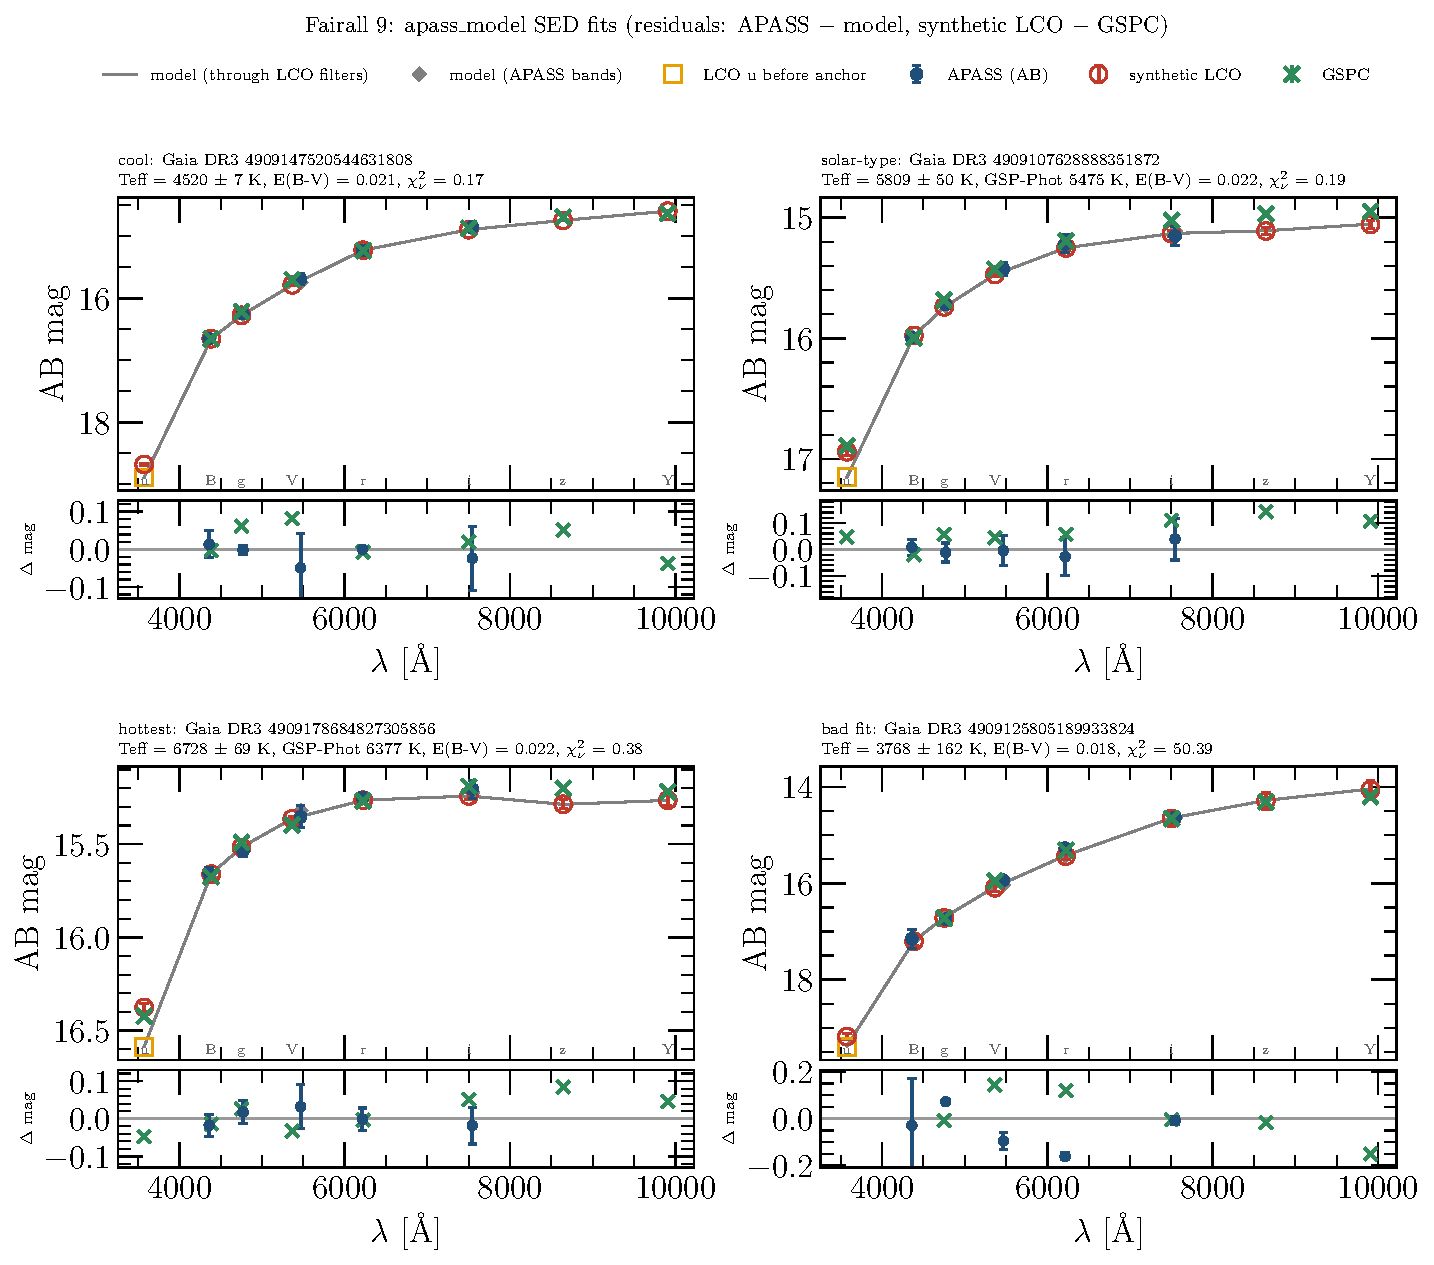
\includegraphics[page=1,width=\textwidth]{figures/reference_sed_example.pdf}
  \caption{SED fits of representative Fairall 9 field stars by the
  \texttt{apass\_model} method. Filled circles: APASS $B\,g\,V\,r\,i$ (AB);
  grey diamonds and line: best-fit reddened BT-Settl/NextGen model, band-averaged
  through the APASS (nominal) and LCO filters; open red circles: synthetic LCO
  magnitudes (\texttt{lco\_*}); orange square: $u$ before the GSPC anchor;
  green crosses: the Gaia DR3 GSPC catalogue value for the same source.
  Lower panels: APASS $-$ model and synthetic LCO $-$ GSPC.}
  \label{fig:refsed-stars}
\end{figure}

\begin{figure}[htbp]
  \centering
  \includegraphics[page=2,width=\textwidth]{figures/reference_sed_example.pdf}
  \caption{Fairall 9 \texttt{apass\_model} summary. (a) Reduced $\chi^2$ of
  the two-parameter fit to five bands; (b) fitted $T_{\rm eff}$ against Gaia
  GSP-Phot; (c) LCO $u$ minus GSPC SDSS $u$ (AB) before (filled) and after (open)
  the per-field anchor, for the stars \texttt{anchor\_u} uses; (d) per-band
  difference from the GSPC catalogue (box: interquartile range).}
  \label{fig:refsed-summary}
\end{figure}
 from docs/ (needs graphicx).
\paragraph{Worked example: Fairall 9.}
The \texttt{apass\_model} fallback (Sec.~\ref{sec:apass_model}) was run on the
Fairall 9 field (APASS DR9 (VizieR II/336), 103 of
152 stars fitted, $E(B-V)_{\rm SF11}=0.022$) and
compared with the production GSPC catalogue (297 quality stars).
Figure~\ref{fig:refsed-stars} shows the fit for representative stars (cool, solar-type, hottest, bad fit);
Fig.~\ref{fig:refsed-summary} summarises the field. The median reduced $\chi^2$
is 0.75. The raw model $u$ is $+0.210\pm0.016$\,mag away from GSPC SDSS $u$ (AB; 27 stars, robust scatter 0.066\,mag) and is shifted by that offset. Median apass\_model $-$ GSPC offsets per LCO band:
u~$+0.019$, B~$-0.040$, g~$+0.032$, V~$+0.009$, r~$-0.004$, i~$+0.024$, z~$+0.036$, Y~$-0.023$\,mag.

\begin{figure}[htbp]
  \centering
  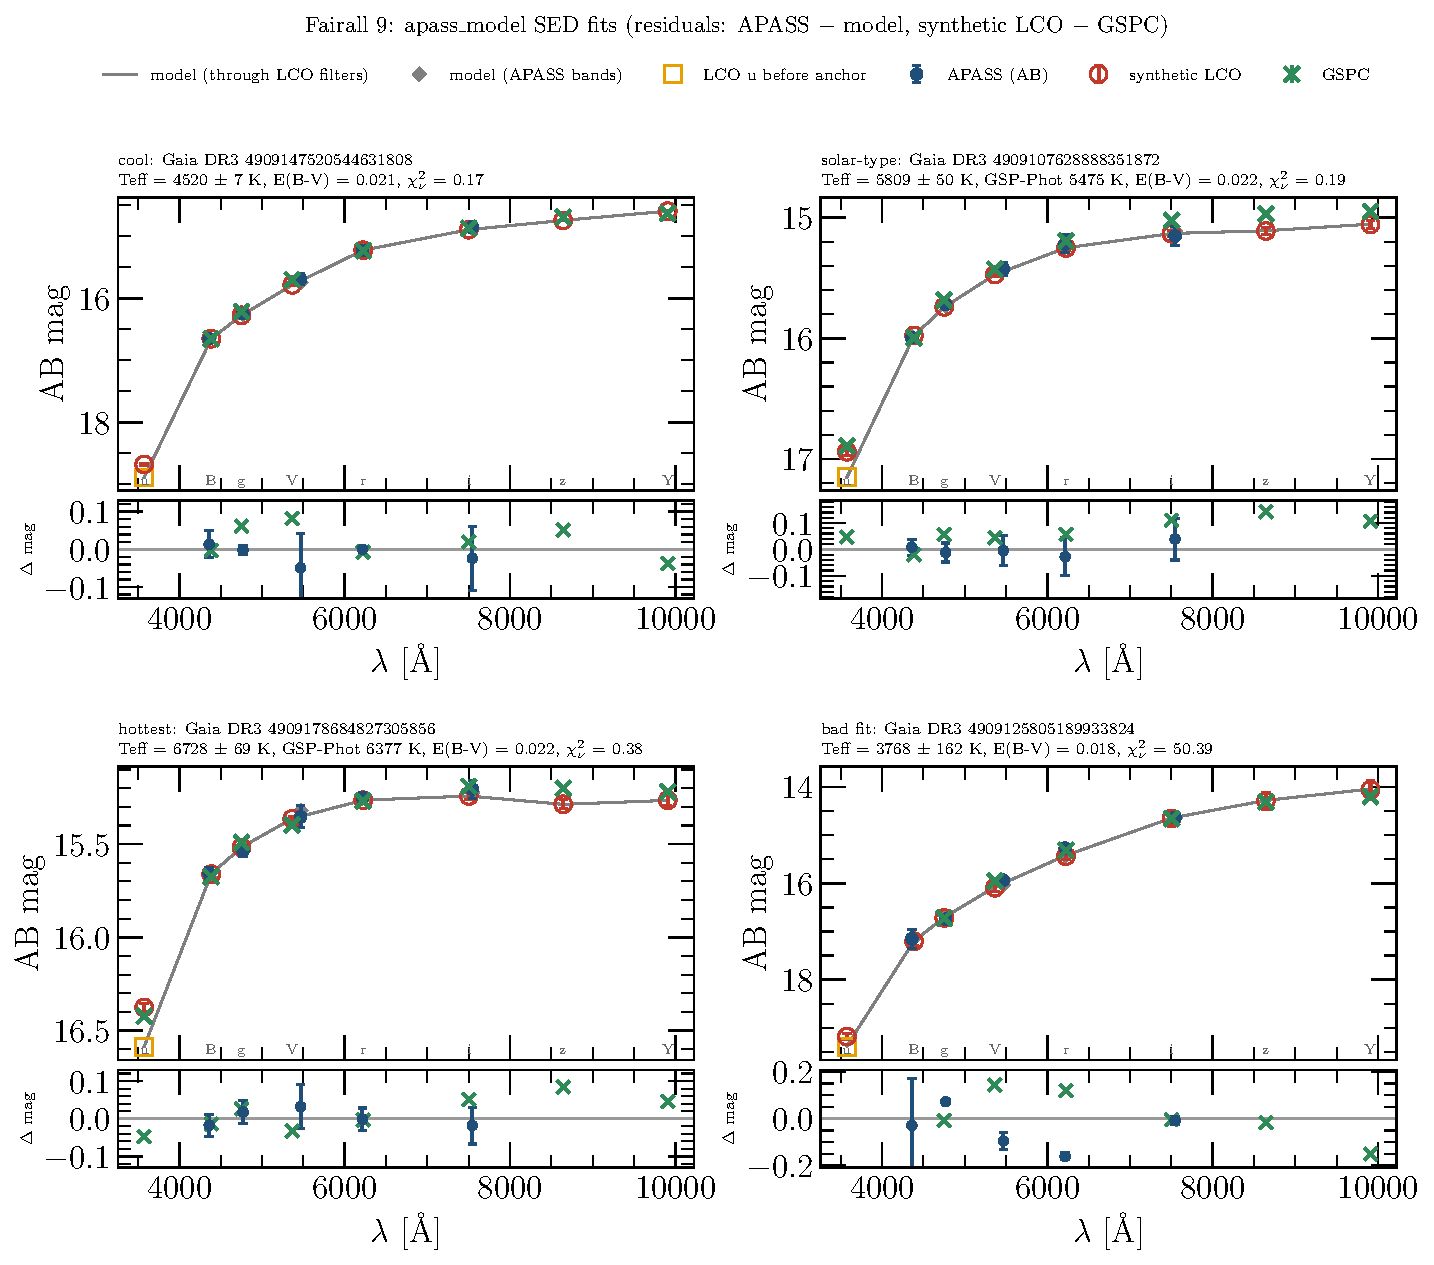
\includegraphics[page=1,width=\textwidth]{figures/reference_sed_example.pdf}
  \caption{SED fits of representative Fairall 9 field stars by the
  \texttt{apass\_model} method. Filled circles: APASS $B\,g\,V\,r\,i$ (AB);
  grey diamonds and line: best-fit reddened BT-Settl/NextGen model, band-averaged
  through the APASS (nominal) and LCO filters; open red circles: synthetic LCO
  magnitudes (\texttt{lco\_*}); orange square: $u$ before the GSPC anchor;
  green crosses: the Gaia DR3 GSPC catalogue value for the same source.
  Lower panels: APASS $-$ model and synthetic LCO $-$ GSPC.}
  \label{fig:refsed-stars}
\end{figure}

\begin{figure}[htbp]
  \centering
  \includegraphics[page=2,width=\textwidth]{figures/reference_sed_example.pdf}
  \caption{Fairall 9 \texttt{apass\_model} summary. (a) Reduced $\chi^2$ of
  the two-parameter fit to five bands; (b) fitted $T_{\rm eff}$ against Gaia
  GSP-Phot; (c) LCO $u$ minus GSPC SDSS $u$ (AB) before (filled) and after (open)
  the per-field anchor, for the stars \texttt{anchor\_u} uses; (d) per-band
  difference from the GSPC catalogue (box: interquartile range).}
  \label{fig:refsed-summary}
\end{figure}
 from docs/ (needs graphicx).
\paragraph{Worked example: Fairall 9.}
The \texttt{apass\_model} fallback (Sec.~\ref{sec:apass_model}) was run on the
Fairall 9 field (APASS DR9 (VizieR II/336), 103 of
152 stars fitted, $E(B-V)_{\rm SF11}=0.022$) and
compared with the production GSPC catalogue (297 quality stars).
Figure~\ref{fig:refsed-stars} shows the fit for representative stars (cool, solar-type, hottest, bad fit);
Fig.~\ref{fig:refsed-summary} summarises the field. The median reduced $\chi^2$
is 0.75. The raw model $u$ is $+0.210\pm0.016$\,mag away from GSPC SDSS $u$ (AB; 27 stars, robust scatter 0.066\,mag) and is shifted by that offset. Median apass\_model $-$ GSPC offsets per LCO band:
u~$+0.019$, B~$-0.040$, g~$+0.032$, V~$+0.009$, r~$-0.004$, i~$+0.024$, z~$+0.036$, Y~$-0.023$\,mag.

\begin{figure}[htbp]
  \centering
  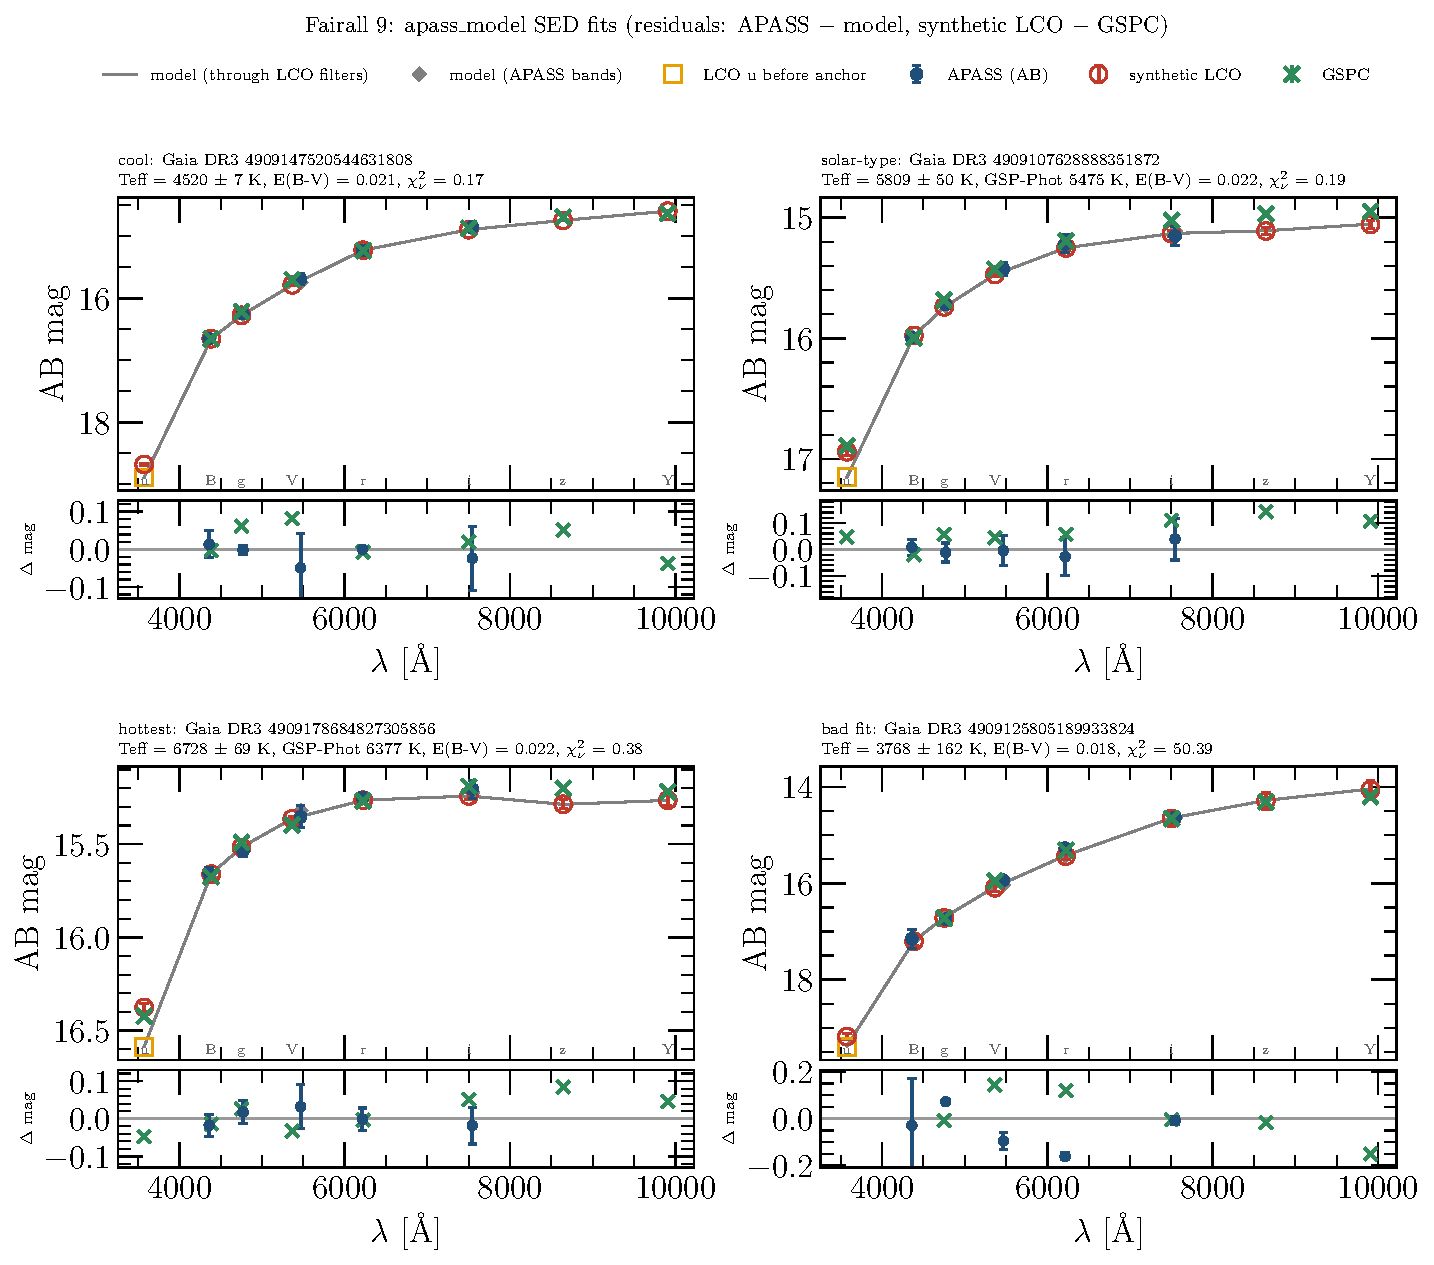
\includegraphics[page=1,width=\textwidth]{figures/reference_sed_example.pdf}
  \caption{SED fits of representative Fairall 9 field stars by the
  \texttt{apass\_model} method. Filled circles: APASS $B\,g\,V\,r\,i$ (AB);
  grey diamonds and line: best-fit reddened BT-Settl/NextGen model, band-averaged
  through the APASS (nominal) and LCO filters; open red circles: synthetic LCO
  magnitudes (\texttt{lco\_*}); orange square: $u$ before the GSPC anchor;
  green crosses: the Gaia DR3 GSPC catalogue value for the same source.
  Lower panels: APASS $-$ model and synthetic LCO $-$ GSPC.}
  \label{fig:refsed-stars}
\end{figure}

\begin{figure}[htbp]
  \centering
  \includegraphics[page=2,width=\textwidth]{figures/reference_sed_example.pdf}
  \caption{Fairall 9 \texttt{apass\_model} summary. (a) Reduced $\chi^2$ of
  the two-parameter fit to five bands; (b) fitted $T_{\rm eff}$ against Gaia
  GSP-Phot; (c) LCO $u$ minus GSPC SDSS $u$ (AB) before (filled) and after (open)
  the per-field anchor, for the stars \texttt{anchor\_u} uses; (d) per-band
  difference from the GSPC catalogue (box: interquartile range).}
  \label{fig:refsed-summary}
\end{figure}
 from docs/ (needs graphicx).
\paragraph{Worked example: Fairall 9.}
The \texttt{apass\_model} fallback (Sec.~\ref{sec:apass_model}) was run on the
Fairall 9 field (APASS DR9 (VizieR II/336), 103 of
152 stars fitted, $E(B-V)_{\rm SF11}=0.022$) and
compared with the production GSPC catalogue (297 quality stars).
Figure~\ref{fig:refsed-stars} shows the fit for representative stars (cool, solar-type, hottest, bad fit);
Fig.~\ref{fig:refsed-summary} summarises the field. The median reduced $\chi^2$
is 0.75. The raw model $u$ is $+0.210\pm0.016$\,mag away from GSPC SDSS $u$ (AB; 27 stars, robust scatter 0.066\,mag) and is shifted by that offset. Median apass\_model $-$ GSPC offsets per LCO band:
u~$+0.019$, B~$-0.040$, g~$+0.032$, V~$+0.009$, r~$-0.004$, i~$+0.024$, z~$+0.036$, Y~$-0.023$\,mag.

\begin{figure}[htbp]
  \centering
  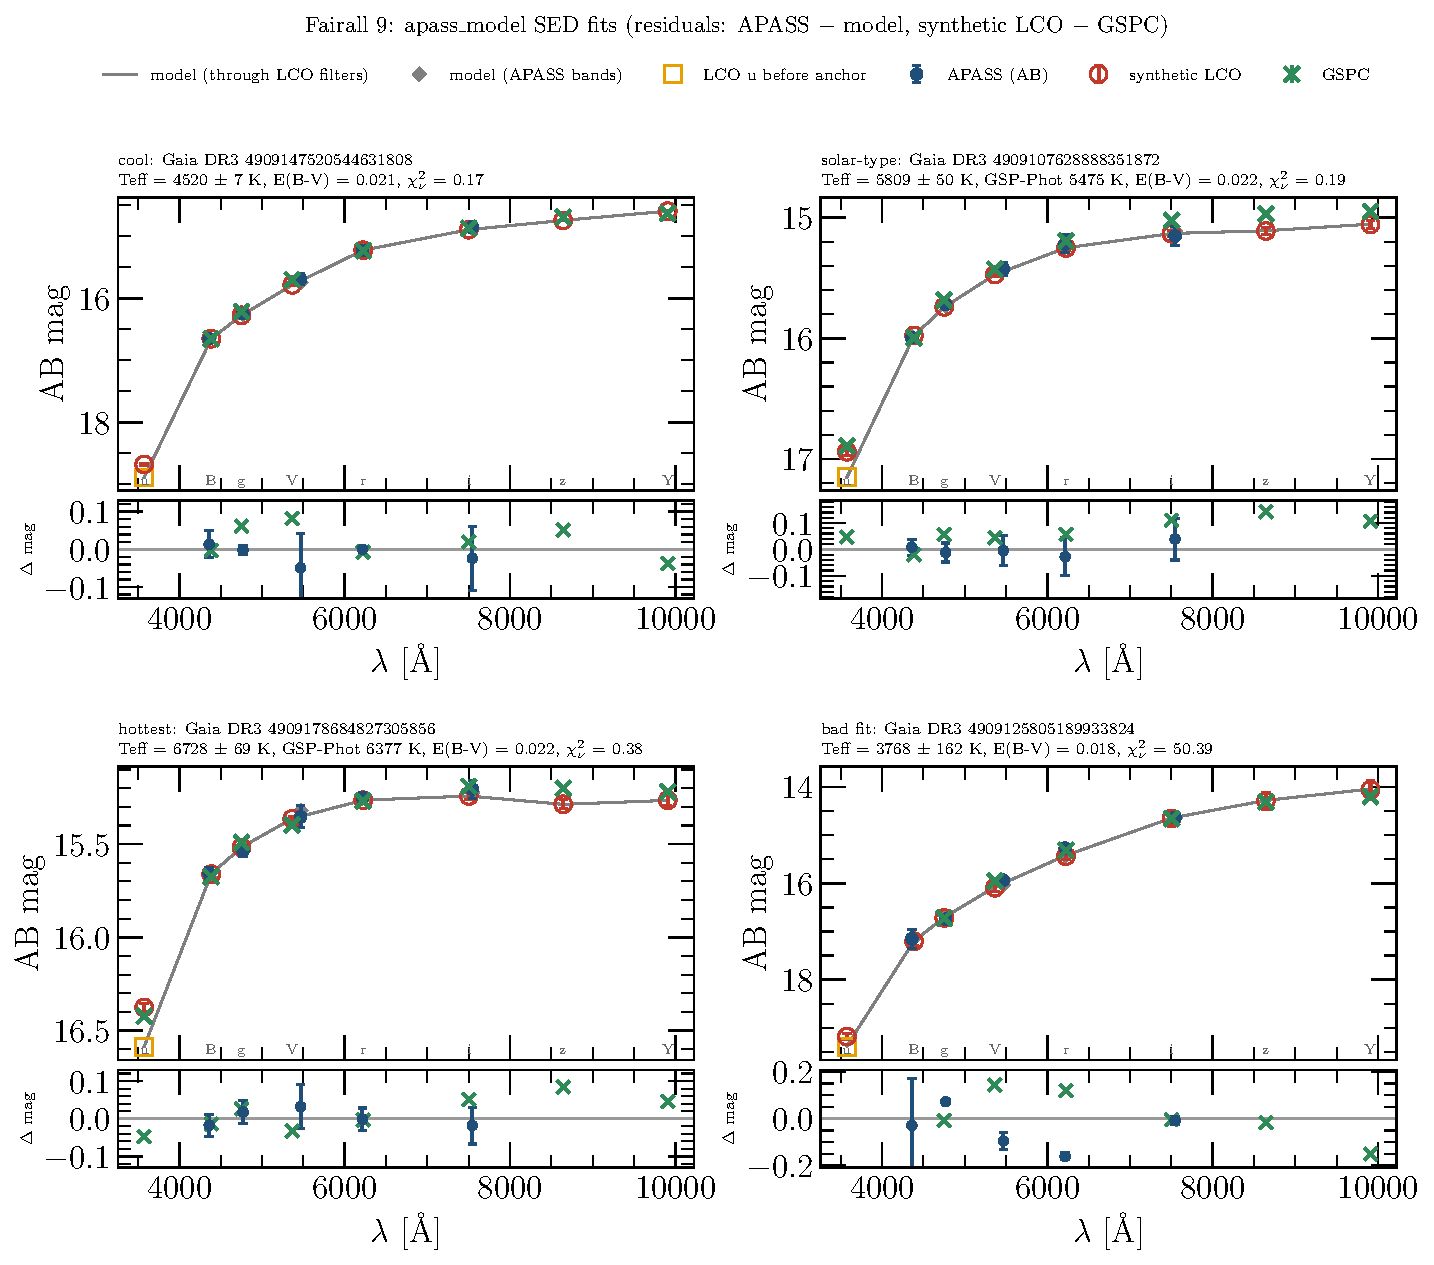
\includegraphics[page=1,width=\textwidth]{figures/reference_sed_example.pdf}
  \caption{SED fits of representative Fairall 9 field stars by the
  \texttt{apass\_model} method. Filled circles: APASS $B\,g\,V\,r\,i$ (AB);
  grey diamonds and line: best-fit reddened BT-Settl/NextGen model, band-averaged
  through the APASS (nominal) and LCO filters; open red circles: synthetic LCO
  magnitudes (\texttt{lco\_*}); orange square: $u$ before the GSPC anchor;
  green crosses: the Gaia DR3 GSPC catalogue value for the same source.
  Lower panels: APASS $-$ model and synthetic LCO $-$ GSPC.}
  \label{fig:refsed-stars}
\end{figure}

\begin{figure}[htbp]
  \centering
  \includegraphics[page=2,width=\textwidth]{figures/reference_sed_example.pdf}
  \caption{Fairall 9 \texttt{apass\_model} summary. (a) Reduced $\chi^2$ of
  the two-parameter fit to five bands; (b) fitted $T_{\rm eff}$ against Gaia
  GSP-Phot; (c) LCO $u$ minus GSPC SDSS $u$ (AB) before (filled) and after (open)
  the per-field anchor, for the stars \texttt{anchor\_u} uses; (d) per-band
  difference from the GSPC catalogue (box: interquartile range).}
  \label{fig:refsed-summary}
\end{figure}
